\pagestyle{empty} % Limpa o cabeçalho e o rodapé
\onehalfspacing % Espaçamento entre-linhas de 1,5
% \hyphenpenalty=10000 % To prevent hyphenation
\pretolerance=10000 % To avoif overful lines
%\selectlanguage{english}
\selectlanguage{brazilian}
\setcounter{ex}{0} % counter for exercises
%\pagenumbering{arabic} % Uncomment this line if you want renumber pages for each chapter
\renewcommand{\chaptername}{Tutorial}
\chapter{Inferência por Verossimilhança Máxima: homologia estática e dinâmica}\label{tut13}
\rhead{\tiny Instituto de Biociências --USP: BIZ0433 - Inferência Filogenética: Filosofia, Método e Aplicações}
\cfoot{\tiny \cc \ccby \ccsa \href{http://creativecommons.org/licenses/by-sa/4.0/}{Creative Commons Attribution-ShareAlike 4.0 International License}}
%\vspace{5pt}
{\large \sc BIZ0433 - Inferência Filogenética: Filosofia, Método e Aplicações.}\par
%{\sc Por \href{http://about.me/machadodj}{Denis Jacob Machado \& Fernando Marques}}\par
\vspace{10pt}
\par
\minitoc % for table of contents within the chapter
\newpage
\section*{}\addcontentsline{toc}{section}{Objetivo}
\onehalfspacing
\vspace*{5pt}
\begin{center}
\emph{\begin{large}Objetivo\end{large}}\label{tut13:Objetivo}
\vspace{2pt}
\end{center}
%% TEXTO DO RESUMO

Este tutorial apresenta implementações de busca sub o critério de verossimilhança máxima (\textbf{ML}) dentro do contexto de homologia estática e dinâmica. O tutorial começa com a apresentação do programa GARLI e como ele pode ser utilizado para análises filogenéticas de homologia estática considerando um único modelo de substituição ou distintos modelos para diferentes partições de dados. Em seguida o tutorial apresenta o uso de POY em análises de \textbf{ML} dentro do contexto de homologia estática e dinâmica. Para POY, o tutorial explora a implementação de \textit{Maximum Avarege Likelihood} (MAL) e \textit{Most Parsimonious Likelihood} (MPL). Adicionamente, este tutorial ilustra como POY pode ser utilizado para seleção de modelos de verossimilhança, bem como os modelos implementados atualmente no programa. Este tutorial deve ser considerado como um elemento introdutório para os conceitos e implementações dos métodos abordados. Maiores detalhes sobre o uso deste critério em análises filogenéticas, a forma de implementação de estratégias heurísticas de buscas mais agressivas, e como aplicar o métodos em diversos caracteres genotípicos e fenotípicos podem ser encontrados na documentação de POY e na literatura referenciada no mesmo. Os arquivos associados a este tutorial estão disponíveis em \url{http://lhe.ib.usp.br/cladistica}. Você pode baixá-los diretamente com o seguinte comando:

\begin{center}
\small \texttt{wget http://lhe.ib.usp.br/downloads/tutorial\_13.zip}\\
\end{center}

\newpage
\pagestyle{fancy} % Inclui o cabeçalho definido no meta.tex
%\pagenumbering{arabic} % Números das páginas em arábicos
\begin{refsection}
\renewcommand*{\finalnamedelim}{\addspace\&\space} % Usar '&' ao invés de 'e'.
%
%% color base pairs
\newcommand{\A}{\textcolor{green}{\textbf{A}}}
\newcommand{\C}{\textcolor{blue}{\textbf{C}}}
\newcommand{\G}{\textcolor{gray}{\textbf{G}}}
\newcommand{\T}{\textcolor{red}{\textbf{T}}}
\newcommand{\gap}{\textcolor{black}{\textbf{-}}}


%%%%%%%%%%%%%%%%%%%%%%%%%%%% HERE TEXT STARTS %%%%%%%%%%%%%%%%%%%%%%%%%%%%

\section{Verrossimilhança: homologia estática em GARLI}\label{tut13:static}
No tutorial anterior exploramos os conceitos relacionados com estimativas de verossimilhança máxima de parâmetros, cálculo de verossimilhança para reconstruções e topologias e seleção de modelos. Desta forma, ficou evidente que o processo lógico de inferência filogenética é o mesmo dentro deste critério de otimalidade, ou seja, topologias são avaliadas quanto ao seu mérito por medidas de verossimilhança e a tolologia que maximiza a probabilidade de obter os dados é selecionada -- da mesma forma que fazemos com o critério de parcimônia.

Neste componente do tutorial iremos explorar os aspectos práticos de inferência sob o critério de verossimilhança máxima em \href{https://code.google.com/archive/p/garli/}{GARLI} \parencite[][]{Zwickl_2006}. Há uma série de outros programas disponíveis para o mesmo propósito (\textit{e.g.}, \href{http://www.iqtree.org/}{IQ-TREE}, \href{http://sco.h-its.org/exelixis/web/software/raxml/index.html}{RAxML}, \href{http://www.atgc-montpellier.fr/phyml/}{PhyML}, \href{http://paup.csit.fsu.edu/downl.html}{PAUP*}, entre outros), mas considero o \href{https://www.nescent.org/wg_garli/Main_Page}{GARLI} um dos mais versáteis disponível atualmente\footnote{Em comparação ao \href{http://www.iqtree.org/}{IQ-TREE}, \href{https://code.google.com/archive/p/garli/}{GARLI} parece explorar mais adequadamente o espaço de topologias, o que pode ser desejável em alguns casos. No entanto, IQ-TREE permite explorar modelos mais complexos de substituição e particionamento de dados e apresentar tempo computacional menor. Caso tenham interesse por esse critério de otimização, sugiro a consulta da documentação do IQ-TREE.}. 

O versatilidade de GARLI está na forma como ele é executado. O programa requer um arquivo de configuração -- usando a mesma lógica que você já usou quando executou o \href{http://www.ib.usp.br/grant/anfibios/researchSoftware.html}{YBIRÁ} -- no qual você define os parâmetros de análise, bem como o arquivo de dados e sufixos de saída em um arquivo de configuração que é lido e executado pelo programa. O exemplo abaixo mostra o conteúdo do arquivo de configuração padrão de GARLI:

\begin{lstlisting}[basicstyle=\scriptsize]
[general]
datafname = arquivo_de_dados.nex
ofprefix = minha_analise
streefname = stepwise
attachmentspertaxon = 10
constraintfile = none
searchreps = 100
outgroup = 1

outputeachbettertopology = 0
outputcurrentbesttopology = 0

enforcetermconditions = 1
genthreshfortopoterm = 5000
scorethreshforterm = 0.001
significanttopochange = 0.01

writecheckpoints = 0
restart = 0

randseed = -1
availablememory = 2000
logevery = 10
saveevery = 100
refinestart = 1
outputphyliptree = 0
outputmostlyuselessfiles = 0
collapsebranches = 1

#linkmodels means to use a single set of model parameters for all subsets.
linkmodels = 1
# subsetspecificrates means to infer overall rate multipliers for each data subset. This is equivalent to *prset ratepr=variable* in MrBayes.
subsetspecificrates = 1
# set for single model, different subset rates (like site-specific rates model in PAUP*)

[model0]
#JC
#number of free parameters: 0
datatype = nucleotide
ratematrix = (a a a a a a)
statefrequencies = equal
ratehetmodel = none
numratecats = 1
invariantsites = none

[master]
bootstrapreps = 0

nindivs = 4
holdover = 1
selectionintensity = 0.5
holdoverpenalty = 0
stopgen = 5000000
stoptime = 5000000

startoptprec = 0.5
minoptprec = 0.01
numberofprecreductions = 2
treerejectionthreshold = 20.0
topoweight = 0.01
modweight = 0.002
brlenweight = 0.002
randnniweight = 0.1
randsprweight = 0.3
limsprweight =  0.6
intervallength = 100
intervalstostore = 5

limsprrange = 6
meanbrlenmuts = 5
gammashapebrlen = 1000
gammashapemodel = 1000
uniqueswapbias = 0.1
distanceswapbias = 1.0

resampleproportion = 1.0
inferinternalstateprobs = 0
\end{lstlisting}

Este arquivo de configuração possui os parâmetros básicos de uma análise que considera um único modelo de substituição para sequências nucleotídicas. Os detalhes sobre cada uma dessas linhas não serão apresentados neste tutorial e o leitor deve consultar a \href{https://molevol.mbl.edu/index.php/GARLI_Configuration_Settings}{documentação do programa} para maiores detalhes. Para os propósitos deste tutorial, iremos comentar apenas algumas linhas, justamente aquelas que são frequentemente modificadas à cada análise:


\begin {myindentpar}{0.3cm}
\begin{enumerate}[\itshape i.]

    \item{Todos os arquivos de configuração do GARLI são divididos em três seções, \texttt{[general]}, \texttt{[model\#]} e \texttt{[master]}.}

    \item{O comando ``\texttt{datafname}'', linha 2, especifica o arquivo de entrada. O GARLI aceita arquivos de dados no formato FASTA ou NEXUS (formato de PAUP*). No entanto, você verá que para algumas análises é necessário o uso do segundo formato. Neste caso, o uso do \texttt{sequencematrix} é recomendável, uma vez que esse programa tem uma opção para exportar seus dados o formato simplificado de NEXUS compatível com o GARLI (veja Tutorial \ref{tut12}).} 

    \item{O comando ``\texttt{ofprefix}'', linha 3, define o prefixo dos arquivos que o GARLI escreverá no diretório de execução. Use um nome curto que lhe informe a análise que está fazendo.} 

    \item{O comando ``\texttt{searchreps}'', linha 7, define o número de réplicas que você deverá fazer em sua análise.} 

    \item{Linhas 30 a 34 especificam como os modelos serão serão considerados pelo GARLI. Neste arquivo de configuração, GARLI irá considerar um único modelo para a partição com uma única taxa para o modelo.}

    \item{Linhas 36 a 44, especifica o modelo de substituição a ser utlizado; nesse caso o modelo JC69 \parencite[][]{Jukes_and_Cantor_1969}. Os modelos disponíveis em GARLI estão no arquivo \texttt{garli\_models.txt} no diretório deste tutorial. O modelo deve ser selecionado anteriormente, veja seção \ref{tut12:first_sec:model} do Tutorial \ref{tut12}.}

\end{enumerate}
\end{myindentpar}


\subsection{GARLI: Single model}\label{tut13:static_garli_single}

Iremos iniciar nossas análises em GARLI considerando um único modelo para os dados, independentemente se eles contém uma ou mais partições. Uma vez editado o arquivo de configuração do GARLI, para iniciar a análise execute:\\

\userprompt{garli garli.conf}\\

Por \textit{default}, o GARLI espera encontrar no diretório de execução um arquivo chamado ``\texttt{garli.conf}''. Se esse arguivo existe, basta executar:\\

\userprompt{garli}\\

No entanto, exceto em execuções paralelas, ou seja, utilizando computadores de auto desempenho ou multi-processados, é recomendável atribuir nomes distintos para os arquivos de configuração. No diretório deste tutorial por exemplo, há o arquivo \texttt{garli\_single.conf}. A execução deste arquivo seria:\\

\userprompt{garli garli\_single.conf}\\

\stepcounter{ex}
\begin{blackBlock}{\textbf{Exercicio 13.\arabic{ex}}}\label{tut13:ex:13.1}

Execute a linha de comando acima.

\end{blackBlock}


A execução desta análise gera os seguintes arquivos de saida:\\

\noindent\texttt{-rw-rw-r--~1~alan~alan~~~~~4357~Jun~~5~15:36~part1.best.all.tre}\\
\texttt{-rw-rw-r--~1~alan~alan~~~~~~766~Jun~~5~15:36~part1.best.tre}\\
\texttt{-rw-rw-r--~1~alan~alan~~~325906~Jun~~5~15:36~part1.log00.log}\\
\texttt{-rw-rw-r--~1~alan~alan~~~108822~Jun~~5~15:36~part1.screen.log}\\

O conteúdo destes arquivos são os seguintes:


\begin {myindentpar}{0.3cm}
\begin{enumerate}[\itshape 1.]

	\item{\texttt{part1.best.all.tre}:} Contém as topologias ótimas encontradas em cada uma das réplicas executadas.

	\item{\texttt{part1.best.tre}:} Contém as melhores topologias encontradas na réplica que resultou na melhor topologia.

	\item{\texttt{part1.log00.log}:} Contém o \textit{log} da execução.

	\item{\texttt{part1.screen.log}:} Contém o \texttt{sdt.err} do GARLI, ou seja, as informações de saida que o programa escreve durante a análise.

\end{enumerate}
\end{myindentpar}

Este último arquivo possui algumas informações que devemos chamar sua atenção. Se você executar a linha de comando:\\

\userprompt{head -n 50 part1.screen.log}\\

Você deverá obter:\\

\scriptsize
\noindent\texttt{\#\#\#\#\#\#\#\#\#\#\#\#\#\#\#\#\#\#\#\#\#\#\#\#\#\#\#\#\#\#\#\#\#\#\#\#\#\#\#\#\#\#\#\#\#\#\#\#\#\#\#}\\
\texttt{PARTITIONING~OF~DATA~AND~MODELS}\\
\texttt{GARLI~data~subset~1}\\
\texttt{~~~~~CHARACTERS~block~\#1~("Untitled~DATA~Block~1")}\\
\texttt{~~~~~Data~read~as~Nucleotide~data,}\\
\texttt{~~~~~modeled~as~Nucleotide~data}\\
\texttt{~~~~~Summary~of~data:}\\
\indent\texttt{~~~~~~~10~sequences.}\\
\indent\texttt{~~~~~~~62~constant~characters.}\\
\indent\texttt{~~~~~~~48~parsimony-informative~characters.}\\
\indent\texttt{~~~~~~~10~uninformative~variable~characters.}\\
\indent\texttt{~~~~~~~120~total~characters.}\\
\indent\texttt{~~~~~~~61~unique~patterns~in~compressed~data~matrix.}\\
\texttt{~~~~~Pattern~processing~required~<~1~second}\\
\texttt{\#\#\#\#\#\#\#\#\#\#\#\#\#\#\#\#\#\#\#\#\#\#\#\#\#\#\#\#\#\#\#\#\#\#\#\#\#\#\#\#\#\#\#\#\#\#\#\#\#\#\#}\\

\normalsize

Os dados acima sumariam as informações de sua matriz de caracteres. Observe que dos 120 caracteres presentes em sua matriz, apenas 61 deles foram condiderados durante a análise. Se você executar a seguinte linha de comando:\\

\userprompt{tail -n 50 part1.screen.log}\\

Você deverá obter:\\

\scriptsize
\noindent\texttt{Completed~10~replicate~search(es)~(of~10).}\\

\texttt{NOTE:~Unless~the~following~output~indicates~that~search~replicates~found~the}\\
\indent\texttt{same~topology,~you~should~assume~that~they~found~different~topologies.}\\
\texttt{Results:}\\
\texttt{Replicate~1~:~-685.0223~~~~~~~}\\
\texttt{Replicate~2~:~-689.6789~~~~~~~}\\
\texttt{Replicate~3~:~-689.6789~~~~~~~~(same~topology~as~2)}\\
\texttt{Replicate~4~:~-686.7873~~~~~~~}\\
\texttt{Replicate~5~:~-684.7616~~~~~~~~(same~topology~as~4)}\\
\texttt{Replicate~6~:~-684.7616~~~~~~~~(same~topology~as~4)}\\
\texttt{Replicate~7~:~-689.6789~~~~~~~~(same~topology~as~2)}\\
\texttt{Replicate~8~:~-684.7039~(best)}\\
\texttt{Replicate~9~:~-685.0222~~~~~~~~(same~topology~as~1)}\\
\texttt{Replicate~10~:~-689.6789~~~~~~~(same~topology~as~2)}\\
\texttt{}\\
\texttt{Parameter~estimates~across~search~replicates:}
\begin{table}[H]
\scriptsize
\begin{tabular}{lcccccccccccc}
 & \texttt{r(AC)} & \texttt{r(AG)} & \texttt{r(AT)} & \texttt{r(CG)} & \texttt{r(CT)} & \texttt{r(GT)} & \texttt{pi(A)} & \texttt{pi(C)} & \texttt{pi(G)} & \texttt{pi(T)} & \texttt{alpha} & \texttt{pinv}\\
\texttt{rep 1:} & \texttt{1} & \texttt{46.32} & \texttt{1} & \texttt{1} & \texttt{46.32} & \texttt{1} & \texttt{0.066} & \texttt{0.039} & \texttt{0.330} & \texttt{0.565} & \texttt{0.175} & \texttt{0.355}\\
\texttt{rep 2:} & \texttt{1} & \texttt{8.028} & \texttt{1} & \texttt{1} & \texttt{8.028} & \texttt{1} & \texttt{0.071} & \texttt{0.040} & \texttt{0.323} & \texttt{0.566} & \texttt{0.159} & \texttt{0.000}\\
\texttt{rep 3:} & \texttt{1} & \texttt{8.032} & \texttt{1} & \texttt{1} & \texttt{8.032} & \texttt{1} & \texttt{0.071} & \texttt{0.040} & \texttt{0.323} & \texttt{0.566} & \texttt{0.159} & \texttt{0.000}\\
\texttt{rep 4:} & \texttt{1} & \texttt{12.68} & \texttt{1} & \texttt{1} & \texttt{12.68} & \texttt{1} & \texttt{0.068} & \texttt{0.040} & \texttt{0.328} & \texttt{0.565} & \texttt{0.292} & \texttt{0.363}\\
\texttt{rep 5:} & \texttt{1} & \texttt{30.39} & \texttt{1} & \texttt{1} & \texttt{30.39} & \texttt{1} & \texttt{0.066} & \texttt{0.039} & \texttt{0.330} & \texttt{0.566} & \texttt{0.076} & \texttt{0.043}\\
\texttt{rep 6:} & \texttt{1} & \texttt{30.41} & \texttt{1} & \texttt{1} & \texttt{30.41} & \texttt{1} & \texttt{0.066} & \texttt{0.039} & \texttt{0.330} & \texttt{0.566} & \texttt{0.076} & \texttt{0.043}\\
\texttt{rep 7:} & \texttt{1} & \texttt{8.036} & \texttt{1} & \texttt{1} & \texttt{8.036} & \texttt{1} & \texttt{0.071} & \texttt{0.040} & \texttt{0.323} & \texttt{0.566} & \texttt{0.159} & \texttt{0.000}\\
\texttt{rep 8:} & \texttt{1} & \texttt{35.09} & \texttt{1} & \texttt{1} & \texttt{35.09} & \texttt{1} & \texttt{0.066} & \texttt{0.039} & \texttt{0.330} & \texttt{0.566} & \texttt{0.073} & \texttt{0.040}\\
\texttt{rep 9:} & \texttt{1} & \texttt{46.43} & \texttt{1} & \texttt{1} & \texttt{46.43} & \texttt{1} & \texttt{0.066} & \texttt{0.039} & \texttt{0.330} & \texttt{0.565} & \texttt{0.175} & \texttt{0.355}\\
\texttt{rep 10:} & \texttt{1} & \texttt{8.015} & \texttt{1} & \texttt{1} & \texttt{8.015} & \texttt{1} & \texttt{0.071} & \texttt{0.040} & \texttt{0.323} & \texttt{0.566} & \texttt{0.159} & \texttt{0.000}\\
\end{tabular}
\end{table}
\texttt{Treelengths:}\\
\texttt{~~~~~~~~~~TL~}\\
\texttt{rep~1:~~482.826}\\
\texttt{rep~2:~~8.665}\\
\texttt{rep~3:~~8.673}\\
\texttt{rep~4:~~32.616}\\
\texttt{rep~5:~~544.587}\\
\texttt{rep~6:~~544.992}\\
\texttt{rep~7:~~8.669}\\
\texttt{rep~8:~~707.949}\\
\texttt{rep~9:~~483.584}\\
\texttt{rep10:~~8.662}\\
\texttt{Saving~final~trees~from~all~search~reps~to~part1.best.all.tre}\\
\texttt{Saving~final~tree~from~best~search~rep~(\#8)~to~part1.best.tre}\\
\normalsize

Estas linhas sumarizam seus resultados após 10 réplicas, dentre as quais a réplica 8\footnote{ Seus resultados podem não ser idênticos a este, pois isso depende de aleatorização, mas devem obedecer a mesma lógica.} resultou na melhor solução com $lnL$ -684.7039. Este arquivo também informa as estimativas dos parâmetros em cada uma das réplicas, tais como as taxas das diversas categorias de subistituição (\textit{i.e.}, \texttt{r(AC)}, \texttt{r(AG)}, \texttt{r(AT)} e etc), as frequências das bases (\textit{i.e.}, \texttt{pi(A)}, \texttt{pi(C)}, \texttt{pi(G)} e \texttt{pi(T)}), o parâmetro $\alpha$ da distribuição gama ($\Gamma$) e a porcentagem dos sítios invariáveis ($I$). Essa tabela é resultado dos parâmetros livres do modelo $HKY+I+\Gamma$ adotado na análise (veja arquivo de configuração).\\


\stepcounter{ex}
\begin{blackBlock}{\textbf{Exercicio 13.\arabic{ex}}}\label{tut13:ex:13.2}

Neste exercício você deverá fazer uma análise sob o critério de verossimilhança máxima em GARLI para os arquivos \texttt{partition1+partition2aln1.nex}, \texttt{partition1+partition2aln2.nex} e \texttt{partition1+partition2aln2.nex} de acordo com os modelos que você selecionou para seus respectivos dados concatenados no Tutorial \ref{tut12}. Para executar esse exercício você deverá:

\end{blackBlock}


\begin {myindentpar}{0.3cm}
\begin{enumerate}[\itshape 1.]

    \item{Editar três os arquivos de configuração de GARLI, um para cada arquivo de dados.}

    \item{Executar o GARLI para cada um dos arquivos de configuração.}

    \item{Sumarizar seus resultados na Tabela \ref{tut13:ex:13.2}, no qual $n$ é o número de caracteres em seu alinhamento, $k$ é o número de parâmetros livres\footnote{ Lembre-se que os parâmetros estimados pelo modelo compreende, a topologia, os comprimentos de cada um dos ramos desta topologia  -- cujo número é dado pela função $(2*t)-3$, no qual $t$ é o número de terminais), e os parâmetros livres do modelo de substituição.} e o $AIC_{c}$ deve ser computado de acordo com as equações \ref{tut12:first_sec:model_aic} e \ref{tut12:first_sec:model_aicc} do Tutorial \ref{tut12}\footnote{ O script aicc.pl pode ser utilizado para obter essa métrica, mas você deverá editar o valor das variáveis de acordo com seus resultados antes de executar o \textit{script}.}.}

\end{enumerate}
\end{myindentpar}


%%%%%%%%%%%%%%%%%%%%%%%%%%% TABELA DE ANÁLISE ML %%%%%%%%%%%%%%%%%%%%%%%%%%% 
%\begin{landscape}
\pagestyle{fancy}
\begin{center}

\begin{longtable}{|l|>{\centering}m{2cm}|>{\centering}m{1cm}|c|>{\centering}m{2cm}|>{\centering}m{2cm} |@{}m{0pt}@{}}
\caption[Análise de modelo único em GARLI.]{Análise de modelo único em GARLI.} \label{tut13:ex:13.2} \\

\hline\hline  \multicolumn{1}{|c|}{\textbf{Dataset}} & \textbf{lnL}  & \textbf{$n$} & \textbf{$k$} & \textbf{$AIC_{c}$} & \textbf{Model} &\\
\endfirsthead

\multicolumn{3}{c}{{\bfseries \tablename\ \thetable{} -- Continuação.}}\\
\hline\hline \textbf{Dataset} & \textbf{lnL}  & \textbf{$n$} & \textbf{$k$} & \textbf{$AIC_{c}$} & \textbf{Model} &\\
\endhead
%\hline \multicolumn{6}{r}{{--continua na próxima página}} \\ \hline
%\endfoot
\hline \hline
%\hline \multicolumn{6}{l}{Consulte a página \url{http://wiki.linuxquestions.org/wiki/Linux_software_equivalent_to_Windows_software}.}
\endlastfoot
\hline \scriptsize\texttt{partition1+partition2aln1.nex} & & & & & &\\
\hline \scriptsize\texttt{partition1+partition2aln2.nex} & & & & & &\\
\hline \scriptsize\texttt{partition1+partition2anl3.nex} & & & & & &\\
\end{longtable}
\end{center}
%\end{landscape}
%%%%%%%%%%%%%%%%%%%%%%%%%%% FIM DA TABELA DE ANÁLISE ML %%%%%%%%%%%%%%%%%%%%%%%%%%



\subsection{GARLI: Partition model}\label{tut13:static_garli_partition}

O GARLI permite que diferentes modelos sejam aplicados à distintas partições de dados. Embora isso seja mais uma das características que conferem versatilidade ao programa, considere que nem sempre -- dentro dos critérios de seleção de modelos em estimativas de verossimilhança máxima -- a adoção de diferentes modelos individuais confere melhores índices à sua análise. Este tutorial irá explorar a implementação dessas análises de forma superficial. Maiores detalhes sobre esse tipo de análise podem ser obtidos em \href{https://molevol.mbl.edu/index.php/Garli_using_partitioned_models}{GARLI partition model documentation}\footnote{ Veja https://molevol.mbl.edu/index.php/Garli\_using\_partitioned\_models}.

Neste tipo de análise, o GARLI requer que os dados estejam no formato NEXUS. Isso é necessário, pois estes arquivos deverão conter um bloco de instrução definindo as partições. Considere por exemplo o arquivo \texttt{partition1+partition2aln1.nex}. Ele é a junção dos arquivos \texttt{partition1.fas} + \texttt{partition2aln1.fas} do Tutorial \ref{tut12}. O primeiro arquivo possui 120 caracteres, ao passo que o alinhamentdo do segundo resultou em 99 caracteres. Portando, no arquivo concatenado \texttt{partition1+partition2aln1.nex}, os caracteres 1 a 120 referem-se à primeira partição, ao passo que os caracteres 121 a 219 referem-se à segunda partição. Sendo este o caso, a primeira etapa de preparação para a análise requer a edição do arquivo \texttt{partition1+partition2aln1\_garli.nex} para que contenha as seguintes linhas:


\begin{lstlisting}[label=tut3:ls1]
BEGIN SETS;
	CHARSET p1 = 1-120;
	CHARSET p2 = 121-219;
	charpartition partitions = s1:p1, s2:p2;
END;
\end{lstlisting}

As linhas 1 e 4 são usadas para abrir e fechar o bloco que define as partições, respectivamente. São definidos dois conjuntos de caracteres, \texttt{p1} e \texttt{p2}, o primeiro de 1 a 120 e o segundo de 121 a 219, linhas 2 e 3. Na linha 4, definimos os \texttt{submodels} de GARLI, \texttt{s1} e \texttt{s2}, para as partições \texttt{p1} e \texttt{p2}, respectivamente. Note que GARLI usa sequencialmente \texttt{s1}, \texttt{s2}, \texttt{s3} e etc para definir os \texttt{submodels}. No entanto, no arquivo de configuração, a sequência de modelos inicia-se no 0; portanto, \texttt{[model0]}, \texttt{[model1]}, \texttt{[model2]} e etc. Este arquivo foi editado e renomeado como \texttt{partition1+partition2aln1\_garli.nex}

Vejamos como ficaria o arquivo de configuração para este arquivo. Considere que, ao selecionar o modelo para os arquivos \texttt{partition1.fas} e \texttt{partition2aln1.fas}, o jModelTest selecionou o modelo de acordo com o $AIC_{c}$. Os modelos selecionados foram $HKY+I+\Gamma$ e $HKY+\Gamma$, respectivamente. Desta forma, esses modelos foram implementados no arquivo \texttt{garli\_p1+2aln1.conf} -- verifique o conteúdo deste arquivo. Observe que além de especificar dois modelos, as linhas 34 a 38 deste arquivo foram modificadas para que o programa considere modelos distintos para cada uma das partições.

Os resultados desta análise estão no diretório do tutorial. A topologia seleciona, com $lnL$ -1475.1010, foi recuperada na réplica \#4 e está escrita no arquivo \texttt{results\_p1+p2aln1.best.tre}. Considere que o particionamento dos modelos confere a essa análise um novo atributo: seu modelo inclui dois modelos de substituição distintos. Para avaliar esse modelo, é necessário calcular o $AIC_{c}$ considerando esses dois modelos de substituição. Recorde que o $AIC_{c}$ é calculado pela seguinte equação:\\

\begin{center}
$AIC_{c} = (-2l + 2k) + \frac{(2k(k-1))}{(n-k-1)}$
\end{center}

Nesta equação, $k$ é o termo que talvez seja menos intuitivo. Como já foi definido, o valor de $k$ é a soma de todos os parâmetros estimados pelo modelo. Ele inclui, a topologia (1), os comprimentos dos ramos ($(2*t)-3$, onde $t$ é o número de terminais; portando, $(2*10)-3 = 17$), e o número de parâmetros livres dos modelos de substituição ($6+5 = 11$; veja comentários nos modelos implementados no arquivo \texttt{garli\_p1+2aln1.conf}). Portanto, o valor de $k$ para esta análise seria $1+17+11 = 29$.\\

Calculado o valor de $k$, o cálculo do $AIC_{c}$ é feito da seguinte maneira:

\begin{center}
$AIC_{c}(p1+2aln1) = (-2*-1475.1010 + 2*29) + \frac{(2*29(29-1))}{(219-29-1)}$
\end{center}

\begin{center}
$AIC_{c}(p1+2aln1) = (2950.202 + 58) + \frac{1624}{192}$
\end{center}

\begin{center}
$AIC_{c}(p1+2aln1) = 3008 + 8.4583 = 3016.6603$\\
\end{center}


\stepcounter{ex}
\begin{blackBlock}{\textbf{Exercicio 13.\arabic{ex}}}\label{tut13:ex:13.3}

Neste exercício você deverá fazer uma análise sob o critério de verossimilhança máxima em GARLI para os arquivos \texttt{partition1+partition2aln2.nex} e \texttt{partition1+partition2aln3.nex} assumindo modelos distintos para cada partiçõas de acordo com os modelos que você selecionou os conjuntos de dados individuais  no Tutorial \ref{tut12}. Para execurar esse exercício você deverá:

\end{blackBlock}


\begin {myindentpar}{0.3cm}
\begin{enumerate}[\itshape 1.]

	\item{Editar os arquivos de dados para implementar os blocos de partições.}
	\item{Editar dois os arquivos de configuração de GARLI, um para cada arquivo de dados.}
	\item{Executar o GARLI para cada um dos arquivos de configuração.}
	\item{Sumarizar seus resultados na Tabela \ref{tut13:ex:13.3}.}
	\item{Responder as perguntas abaixo:}

\end{enumerate}
\end{myindentpar}


%%%%%%%%%%%%%%%%%%%%%%%%%%% TABELA DE ANÁLISE ML %%%%%%%%%%%%%%%%%%%%%%%%%%% 
%\begin{landscape}
\pagestyle{fancy}
\begin{center}

\begin{longtable}{|l|>{\centering}m{2cm}|>{\centering}m{1cm}|c|>{\centering}m{2cm}|>{\centering}m{2cm} |@{}m{0pt}@{}}
\caption[Análise de modelo particionado em GARLI.]{Análise de modelo particionado em GARLI.} \label{tut13:ex:13.3} \\

\hline\hline  \multicolumn{1}{|c|}{\textbf{Dataset}} & \textbf{lnL}  & \textbf{$n$} & \textbf{$k$} & \textbf{$AIC_{c}$} & \textbf{Model} &\\
\endfirsthead

\multicolumn{3}{c}{{\bfseries \tablename\ \thetable{} -- Continuação.}}\\
\hline\hline \textbf{Dataset} & \textbf{lnL}  & \textbf{$n$} & \textbf{$k$} & \textbf{$AIC_{c}$} & \textbf{Model} &\\
\endhead
%\hline \multicolumn{6}{r}{{--continua na próxima página}} \\ \hline
%\endfoot
\hline \hline
%\hline \multicolumn{6}{l}{Consulte a página \url{http://wiki.linuxquestions.org/wiki/Linux_software_equivalent_to_Windows_software}.}
\endlastfoot
\hline \scriptsize\texttt{partition1+partition2aln1.nex} & -1475.1010 & 219 & 29 & 3016.6603 & \tiny\texttt{$HKY+I+\Gamma$/$HKY+\Gamma$} &\\
\hline \scriptsize\texttt{partition1+partition2aln2.nex} & & & & & &\\
\hline \scriptsize\texttt{partition1+partition2anl3.nex} & & & & & &\\
\end{longtable}
\end{center}
%\end{landscape}
%%%%%%%%%%%%%%%%%%%%%%%%%%% FIM DA TABELA DE ANÁLISE ML %%%%%%%%%%%%%%%%%%%%%%%%%%

\begin {myindentpar}{0.3cm}
\begin{enumerate}[\itshape 1.]

	\item{De acordo com o critério de $AIC_{c}$, qual análise você selecionaria? Justifique.}

\begin{center}
\line(1,0){400}\\
\line(1,0){400}\\
\line(1,0){400}\\
\end{center}



	\item{Seu resultado é dependente do critério de otimalidade? Justifique.}

\begin{center}
\line(1,0){400}\\
\line(1,0){400}\\
\line(1,0){400}\\
\end{center}

\end{enumerate}
\end{myindentpar}



\section{Verrossimilhança: homologia dinâmica em POY}\label{tut13:dynamic} 
 
 Para dados sujeitos a alinhamento\footnote{Texto baseado na documentação de POY \parencite[][]{VaronETAL_2014}}, a implementação de análises de homologia dinâmica também é possível. O programa POY permite a implementação dessas análises. A análise dos dados moleculares sob verossimilhança em POY, considerando dados pré-alinhados (homologia estática) ou não (homologia dinâmica), pode ser significativamente mais demorada do que análises sob o critério de otimalidade de parcimônia. Portanto, é necessário adotar algumas estratégias que visem reduzir o tempo computacional sob verossimilhança. Uma das estratégias mais efetivas -- embora com algumas deficiências -- é iniciar a análise com parâmetros de busca menos complexos, adotando até mesmo parcimônia como critério de otimalidade inicial, e coletar topologias que seriam refinadas sob o critério de verossimilhança no qual se adota procedimentos mais complexos de cômputo até que se atinja o nível de agressividade de busca heurística desejado. Veja abaixo alguns componentes -- ou procedimentos -- que podem ser manipulados durante sua análise dentro do contexto exposto acima:

\begin {myindentpar}{0.3cm}
\begin{enumerate}[\itshape i.]
	\item{\textbf{Topologias candidatas sob o critério de parcimônia:}}\label{tut13:dynamic:par}

Esta etapa da análise começa com a construção e busca inicial (de complexidade arbitrária) sob parcimônia antes de adotar o critério de verossimilhança na escolha de modelos e diagnose de topologias. Este procedimento economiza tempo, evitando RAS e refinamento (\textit{i.e.}, TBR, SPR, \textit{tree-fusing}, entre outros) sob o critério de verossimilhança -- o que demanda enorme quantidade de cálculo. Um problema potencial desta estratégia heurística é que uma ou mais topologia considerada ótima sob o critério de parcimônia pode estar longe no espaço de árvores de uma topologia considerada ótima sob o critério de verossimilhança. Por esse motivo, é recomendável que sejam adotadas estratégias de refinamento (via algoritmos de rearranjo -- \textit{e.g.}, TBR -- ou até mesmo algoritmos genéticos -- \textit{e.g., tree-fusing}) após a adoção do critério de verossimilhança.

	\item{\textbf{Estimativa aproximada (grosseira) de parâmetros:}}\label{tut13:dynamic:gran_par}

A granularidade da estimativa dos parâmetros do modelo pode ser manipulada durante a análise. Por exemplo, durante os rearranjos sob o critério de verossimilhança, todos os comprimentos de ramos (independentemente da distância entre a quebra e a reconexão) são re-otimizados, o mesmo ocorrendo para os parâmetros do modelo a cada rearranjo. O tempo de execução pode ser minimizado executando a otimização do modelo somente se o custo de um rearranjo está dentro de um número limite em comparação ao melhor custo encontrado até o momento, ou pela otimização do comprimento de ramos em determinadas condições -- distância da quebra e da reconexão em cada rearranjo. Esta estratégia é adotada, por exemplo, pelo programa RAxML - Randomized Axelerated Maximum Likelihood \parencite[][]{Stamatakis_2014} que inicia as buscas heurísticas adotando o modelo GTRCAT \footnote{Esse é um algoritmo de aproximação, veja \url{http://sco.h-its.org/exelixis/resource/download/NewManual.pdf}} e durante o processo de refinamento adota o modelo GTRGAMMA que otimiza mais agressivamente os parâmetros do modelo.

	\item{\textbf{Granularidade na precisão de cálculos (\textit{Floating point granularity}):}}\label{tut13:dynamic:gran_float}

A precisão das casas decimais pode ser diminuida durante os cálculos para limitar o tempo gasto em otimizar os valores dos parâmetros durante os rearranjos ou até mesmo durante a transformação dos caracteres em verossimilhança. A escolha da granularidade atua -- limitando -- na precisão dos cálculos e no número de iterações realizadas durante o processo de estimativa de parâmetros. Um problema potencial desta estratégia heurística é que a redução da precisão (\textit{coarse granularity}) pode afetar negativamente as análises para as quais várias topologias e/ou comprimentos ramos são muito similares, ou até igualmente ótimos existam. Adicionalmente, os índices de verossimilhança -- ou \textit{likelihood scores} -- sob baixa precisão não são comparáveis com aqueles obtidos em outros programas que adotam o mesmo critério de otimalidade. Neste caso, a otimização completa deve ser realizada na topologia final.

	\item{\textbf{Cronograma de Otimização:}}\label{tut13:dynamic:string}

Essa estratégia manipula a etapa na qual é aplicado maior rigor na otimização dos parâmetros do modelo. Por exemplo, sob o rearranjo tradicional sob o critério de verossimilhança, todos os comprimentos de ramo (independentemente da distância entre quebra e reconexão) e os parâmetros do modelo são recalculados para cada topologia. Pode-se diminuir o tempo computacional especificando quando tal rigor deve ser aplicado; otimizando os parâmetros do modelo somente se o custo de um rearranjo está dentro de um limite pré-especificado de acordo com a topologia ótima obtida até então, ou otimizando os comprimentos dos ramos dentro de uma distância específica entre quebra e reconexão para cada rearranjo. O problema potencial com esta estratégia heurística é definir a priori quando este rigor deve ser aplicado e é bem provável que estas propriedades são altamente dependente dos dados em mãos.

	\item{\textbf{Estratégias de rearranjo:}}\label{tut13:dynamic:refs}

O número de topologias visitadas durante a etapa de refinamento por algoritmos de rearranjo (que variam entre NNI e TBR) pode ser restringido nos estágios iniciais de busca. Esta abordagem minimiza o número de cálculos durante os rearranjos, enquanto que o aumento da granularidade restringe o tempo gasto em um determinado cálculo. Uma vez que topologias foram selecionadas e supostamente estejam perto da solução ótima, pode-se proceder com buscas e estimativa de parâmetros mais agressivas. O problema potencial desta estratégia é similar ao uso de topologias iniciais estimadas pelo critério de parcimônia e o usuário pode ficar restrito a um ótimo local limitado pelo espaço explorado durante o refinamento por algoritmos de rearranjo.

\end{enumerate}
\end{myindentpar}

Existem outras possibilidades de estratégias heurísticas, incluindo alternância entre os critérios de otimalidade em caracteres estáticos (transformações alternadas entre critérios de verossimilhança e parcimônia para caracteres estáticos), entre as variações de um mesmo critério de otimalidade (entre MPL e MAL), ou entre premissas para caracteres (entre quatro e cinco estados de caráter para um determinado modelo).

\subsection{Formas de implementação}\label{tut13:ml} 

O POY permite o uso de dois critérios de verossimilhança em inferência filogenética. A primeira delas seria a \textit{Maximum Average Likelihood} (MAL) na análise de dados quantitativos com alfabetos de qualquer tamanho (\textit{i.e.}, sequências nucleotídicas, aminoácios, entre outros) para \textbf{sequências alinhadas}\footnote{MAL pode ser aplicado em sequências não alinhadas, porém requer que os caracteres sejam transformados inicialmente em caracteres estáticos, veja abaixo. O cálculo de MAL sob homologia dinâmica seria computacionalmente impraticável (Wheeler, pers. comm.).}, considerando \textit{gaps} como dados lacunares (\textit{i.e., missing data}) ou como um quinto estado de caráter. A segunda seria a \textit{Most Parsimonious Likelihood} (MPL) que pode ser aplicada aos mesmos tipos de dados, além de sequências não alinhadas (busca heurística MPL/DO). Adicionalmente, o POY avalia e permite a aplicação de uma série de modelos de substituição (14) além de considerar INDELs (\textit{i.e.}, inserções e deleções) nesses modelos.

%%%%%%%%%%%%%%%%%%%%%%%%%%%% SELEÇÃO DE MODELOS %%%%%%%%%%%%%%%%%%%%%%%%%%%% 

\subsection{Seleção de modelos de verossimilhança em POY}\label{tut13:ml:modeltest}
% this should be a section in later versions

Como discutido no Tutorial \ref{tut12}, este prodedimento define e seleciona o modelo estocástico de evolução (modelo de substituição) que otimiza a função de verossimilhança. POY, como na maioria dos programas que implementa esse critério de otimalidade, aplica um modelo homogêneo que estima as taxas de substituição utilizando uma única matriz de probabilidades ao longo de toda topologia. A adoção do critério de verosimilhança requer a adoção de um modelo de substituição de caracteres.
%Nos exemplos vistos acima, assumimos que o modelo GTR+$\Gamma$ \parencite[][]{Tavare_1986}, seria o mais apropriado para os dados. 
Toda análise de verossimilhança requer justificativa para a adoção de modelos. Estas justificativas residem na aplicação de critérios (\textit{e.g.}, LRT, AIC, AICc, BIC, entre outros) que visam avaliar a relação entre nível de parametrização do modelo e a otimização da função de verossimilhança \parencite[veja breve discussão e referências em][; Tutorial \ref{tut12}]{Darriba_and_Posada_2015}.

Os modelos de substituição disponíveis em POY incluem JC69/Neyman, F81, K2P/K80, F84, HKY85, TN93, e GTR, todos sob os quais pode-se ainda implementar categorias de taxa heterogêneas de substituição com a distribuição Gama ($\Gamma$) (Figura \ref{tut13:fig:models}). POY não considera a proporção de sítios ivariávels ($I$) como um parâmetro do modelo, uma vez que ele tecnicamente estaria contemplado na distribuição Gama ($\Gamma$). A seleção de modelos pode feita de forma automatizada, cabendo ao usuário a escolha de um critério dentre os três disponíveis em POY: AIC, AICc and BIC \parencite[para a definição de BIC, veja][]{Darriba_and_Posada_2015}.

%%%%%%%%%%%%%%%%%%%%%%%%%%% FIGURA MODELS IN POY%%%%%%%%%%%%%%%%%%%%%%%%%%%
%  \vspace{-1em}
  \begin{figure}[h!]
    %\ffigbox[\FBwidth]
      {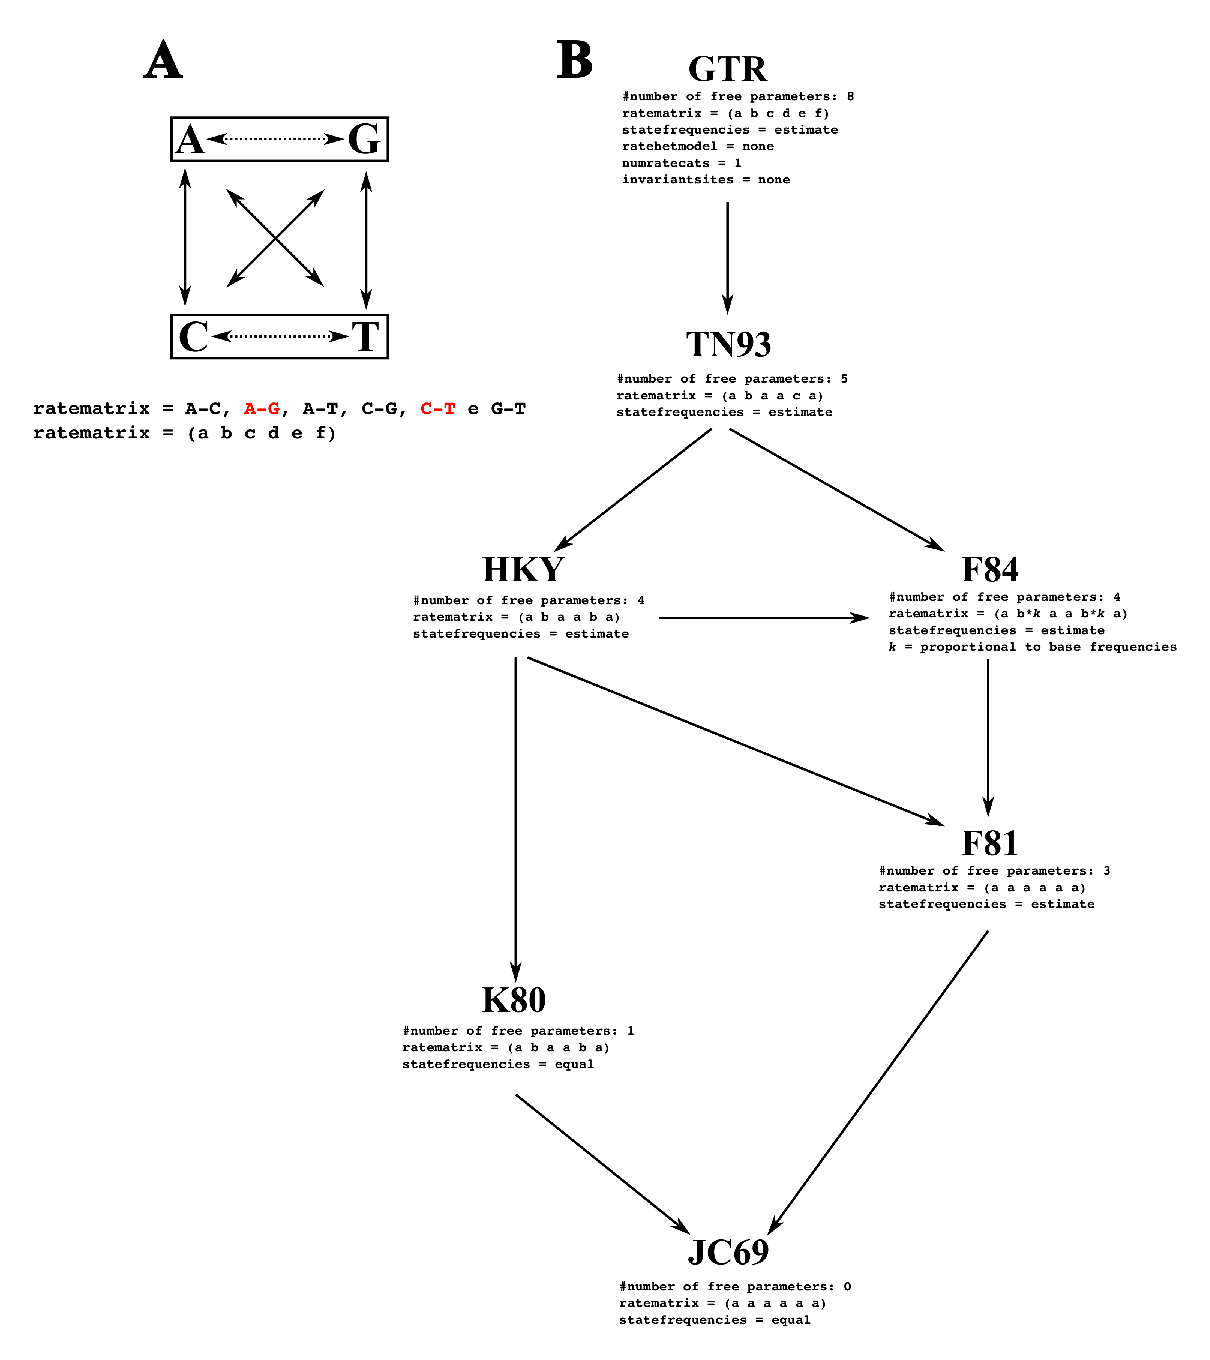
\includegraphics[scale=0.8]{figures/tut13/models.eps}}
    {\caption[Modelos de substituição avaliados em POY]{Modelos de substituição avaliados em POY. \textbf{A}. Seis substituições possíveis para nucleotídeos. Tranformações pontinhadas referem-se a transições, demais transformações são transversões. Estas seis transformações define os elementos das matrizes de substituições (\texttt{ratematrix} em Garli), cujas transformações em vermelho representam transições. A representação tradicional dessas transformações são expressas pelas letras \textit{a}--\textit{f}. \textbf{B}. Relação hierárquica dos modelos de substituição avaliados em POY. Para cada modelo é informado o número de parâmetros livres (\textit{i.e.}, aqueles que são estimados durante a otimização da função de verossimilhança). Considere que para cada um desses modelos, POY considera taxas heterogêneas de substituição de acordo com 0 a 8 categorias da distribuição Gama ($\Gamma$).\footnote{A implementação de \textit{gaps} como quinto estado não está representada nesta ilustração.}}\label{tut13:fig:models}}
  \end{figure}

%%%%%%%%%%%%%%%%%%%%%%%%%%% FIM DA FIGURA MODELS IN POY %%%%%%%%%%%%%%%%%%%%%
\scriptsize
\begin{lstlisting}[caption= conteúdo do arquivo \texttt{model\_test\_part1.poy}.,label=tut13:modsel:model_test_mal]

(*MAL Analysis: Partitions and Model Selection*)
read(prealigned:("partition1.fas",tcm:(1,1)))
build(100)
swap()
select(best:1)
transform(likelihood:(aicc:"part1_AICc.txt",rates:gamma:(4), priors: estimate,mal))
swap()
report("part1_LK.tre",trees:(branches),"part1_LK_lkm.txt",lkmodel)
exit()

\end{lstlisting}
\normalsize

A forma de implementação da seleção de modelos em POY é relativamente simples. Considere, por exemplo o \textit{script} \ref{tut13:modsel:model_test_mal}. Na linha 1, o \textit{script} lê os dados do arquivo \texttt{partition1.fas} e atribui peso 1 para todas as transformações. Posteriormente, linha 2 e 3, ele faz 100 RAS+TBR, cuja a melhor topologia é selecionada na linha 5. Observem que as buscas e seleção foram feitas aqui sob o critério de parcimônia. A linha 6 transforma o critério de otimalidade para verossimilhança, mais precisamente \textit{Maxinum Average Likelihood} (veja abaixo), e inicia o teste de modelos adotando $AIC_{c}$ como critério de seleção. O modelo de verossimilhança considera 4 categorias de taxas de substituições, distribuição Gamma ($\Gamma$), e os parâmetros livres dos modelos deverão ser estimados durante a análise. Posteriormente, o POY adota o melhor modelo sob esse critério de otimalidade e faz uma busca por \texttt{swap} cujos resultados, topologias e modelo, são impressos em seus respectivos arquivos de saida. Observe que esse \textit{script} executa a seleção de modelo e faz buscas -- embora muito heurística -- em uma única análise.

A execução do \texttt{model\_test\_part1.poy} resulta em 3 arquivos. O arquivo \texttt{part1\_AICc.txt} contém uma tabela comparativa dos modelos analisados cujo resultado é apresentado na Tabela \ref{tut13:table:modsel}. O arquivo \texttt{part1\_LK\_lkm.txt} detalha o modelo de substituição resultado da busca. Finalmente, o arquivo \texttt{part1\_LK.tre} contém a topologia com seus respectivos comprimentos de ramos resultado da análise.

\scriptsize
\begin{lstlisting}[caption= conteúdo do arquivo \texttt{model\_test\_part2a1mi.poy}.,label=tut13:modsel:model_test_mal_gap]
(*ML Analysis: Partitions and Model Selection*)
read("partition2a1.fas")
transform(tcm:(1,1))
search(max_time:0:0:02)
select(best:1)
transform(static_approx)
transform(likelihood:(aicc:"part2a1mi_AICc.txt",rates:gamma:(4), priors:estimate, gap:missing, mal))
swap()
report("part2a1mi_LK.tre",trees:(branches),"part2a1mi_LK_lkm.txt",lkmodel)
exit()
\end{lstlisting}
\normalsize

No exemplo anterior, os dados iniciais encontravam-se pré-alinhados. O \textit{script} \ref{tut13:modsel:model_test_mal_gap} executa as mesmas análise do \textit{script} anterior para dados não alinhados. Se compararmos os dois \textit{scripts} notaremos que o segundo (\textit{script} \ref{tut13:modsel:model_test_mal_gap}) lê e transforma os dados iniciais de forma diferente (linhas 2 e 3). Posteriormente, na linha 4, ele faz uma busca pelo comando \texttt{search} por dois minutos e seleciona uma árvore ótima, linha 5. Na linha 7, os caracteres que até então eram tratados como homologia dinânica são transformados em caracteres estáticos (\texttt{transform(static\_approx)}) -- essa transformação é necessária pois o POY só faz MAL sob homologia estática. Em seguida, POY inicia a seleção de modelos como no \textit{script} anterior, mas considerando gaps como dados lacunares (\texttt{gap:missing}) -- da mesma forma que o GARLI. O POY permite três tratamentos diferentes para INDELs. Eles podem ser tratados como ``\textit{missing data}'' e como tal não influenciam o cálculo de verossimilhança; podem ser tratados como caracteres (\texttt{gap:character}), neste caso inserções e deleções de A, C, G e T são tratadas individualmente como diferentes eventos e estimados independentemente; e finalmente, eles podem ser tratados de maneira conjugada (\texttt{gap:coupled}), e neste caso INDELs como um todo são tratados como um único parâmetro.\\


%%%%%%%%%%%%%%%%%%%%%%%%%%% TABELA DE SELEÇAO DE MODELOS EM POY %%%%%%%%%%%%%%%%%%%%%%%%%%% 
%\begin{landscape}
%\pagestyle{fancy}
\begin{center}
\scriptsize 
\begin{table}[H]
\caption[Seleção de modelos em POY]{Exemplo de arquivo de saída de POY para a seleção de modelos utilizando $AIC_{c}$ mostrando os valores de verosimilhança para cada modelo avaliado. Colunas representam, modelo avaliado, \textit{log} negativo da verossimilhança ($-L$), número de parâmetros estimados -- inclui parâmetros livres do modelo + número de comprimentos de ramos (= $2t-3$, onde $t$ é o número de terminais) + topologia -- ($K$), número de caracteres ($n$), valores de $AIC_{c}$, diferença entre valores de $AIC_{c}$ ($\Delta$), pesos de Akaike ($\omega$) e peso acumulado de Akaike (Cum($\omega$)).  Neste exemplo, o modelo HKY+$\Gamma$ possui o maior valor teórico de informação e seria o modelo selecionado.} \label{tut13:table:modsel}

\begin{tabular}{llllllll}
\hline
\multicolumn{1}{c}{\textbf{Modelo}}&
\multicolumn{1}{c}{\textbf{$-lnL$}}&
\multicolumn{1}{c}{\textbf{$K$}}&
\multicolumn{1}{c}{\textbf{$n$}}&
\multicolumn{1}{c}{\textbf{$AIC_{c}$}}&
\multicolumn{1}{c}{\textbf{$\Delta$ $AIC_{c}$}}&
\multicolumn{1}{c}{\textbf{$\omega$}}&
\multicolumn{1}{c}{\textbf{Cum($\omega$)}}\\
\hline\hline

HKY+$\Gamma$ & \scriptsize 699.988278259 & \scriptsize 22 & \scriptsize 120 & \scriptsize 1454.40954621 & \scriptsize 0. & \scriptsize 0.83608261736 & \scriptsize 0.83608261736 \\
F84+$\Gamma$ & \scriptsize 701.73534071 & \scriptsize 22 & \scriptsize 120 & \scriptsize 1457.90367111 & \scriptsize 3.49412490153 & \scriptsize 0.145716795637 & \scriptsize 0.981799412997 \\
TN93+$\Gamma$ &\scriptsize  702.530154326 & \scriptsize 23 & \scriptsize 120 & \scriptsize 1462.56030865 & \scriptsize 8.15076244343 &\scriptsize  0.0142014803771 & \scriptsize 0.996000893374 \\
F81+$\Gamma$ & \scriptsize 707.445080336 & \scriptsize 21 & \scriptsize 120 & \scriptsize 1466.3187321 & \scriptsize 11.9091858917 & \scriptsize 0.00216871426416 & \scriptsize 0.998169607638 \\
GTR+$\Gamma$ & \scriptsize 699.780583091 & \scriptsize 26 & \scriptsize 120 & \scriptsize 1466.65794038 & \scriptsize 12.2483941669 & \scriptsize 0.00183039236205 & \scriptsize 1. \\
F81 & \scriptsize 803.540920474 & \scriptsize 20 & \scriptsize 120 & \scriptsize 1655.56668943 & \scriptsize 201.157143224 & \scriptsize 1.74393601054e-44 & \scriptsize 1. \\
F84 & \scriptsize 812.286360077 & \scriptsize 21 & \scriptsize 120 & \scriptsize 1676.00129158 & \scriptsize 221.591745375 & \scriptsize 6.37108014702e-49 & \scriptsize 1. \\
K81+$\Gamma$ & \scriptsize 836.480712188 & \scriptsize 19 & \scriptsize 120 & \scriptsize 1718.56142438 & \scriptsize 264.151878168 & \scriptsize 3.65088083617e-58 & \scriptsize 1. \\
JC69+$\Gamma$ & \scriptsize 842.281419936 & \scriptsize 18 & \scriptsize 120 & \scriptsize 1727.3351171 & \scriptsize 272.925570891 & \scriptsize 4.54165865543e-60 & \scriptsize 1. \\
TN93 & \scriptsize 870.744628139 & \scriptsize 22 & \scriptsize 120 & \scriptsize 1795.92224597 & \scriptsize 341.512699759 & \scriptsize 5.80374993199e-75 & \scriptsize 1. \\
HKY & \scriptsize 875.31326933 & \scriptsize 21 & \scriptsize 120 & \scriptsize 1802.05511009 & \scriptsize 347.64556388 & \scriptsize 2.70379754075e-76 & \scriptsize 1. \\
GTR & \scriptsize 903.181048846 & \scriptsize 25 & \scriptsize 120 & \scriptsize 1870.19188493 & \scriptsize 415.782338718 & \scriptsize 4.32774342593e-91 & \scriptsize 1. \\
K81 & \scriptsize 944.292608696 & \scriptsize 18 & \scriptsize 120 & \scriptsize 1931.35749462 & \scriptsize 476.947948412 & \scriptsize 2.26109140474e-104 & \scriptsize 1. \\
JC69 & \scriptsize 955.127444482 & \scriptsize 17 & \scriptsize 120 & \scriptsize 1950.25488896 & \scriptsize 495.845342756 & \scriptsize 1.78156255514e-108 & \scriptsize 1. \\\hline

\end{tabular}
\end{table}

\end{center}
%\end{landscape}

%%%%%%%%%%%%%%%%%%%%%%%%%%% FIM DA TABELA DE SELEÇAO DE MODELOS EM POY %%%%%%%%%%%%%%%%%%%%%%%%%%
\normalsize
\stepcounter{ex}
\begin{blackBlock}{\textbf{Exercicio 13.\arabic{ex}}}\label{tut13:ex:13.4}

Neste exercício você deverá fazer uma análise sob o critério de verossimilhança máxima em POY para o arquivo \texttt{partition2aln1.fas} que você gerou no Tutorial \ref{tut12} implementando os três tratamentos de gaps possíveis no programa. Para executar esse exercício você deverá:

\end{blackBlock}



%%%%%%%%%%%%%%%%%%%%%%%%%%% TABELA DE ANÁLISE ML %%%%%%%%%%%%%%%%%%%%%%%%%%% 
%\begin{landscape}
\pagestyle{fancy}
\begin{center}

\begin{longtable}{|l|>{\centering}m{2cm}|>{\centering}m{1cm}|c|>{\centering}m{2cm}|>{\centering}m{2cm} |@{}m{0pt}@{}}
\caption[Tratamento de gaps em POY.]{Análise de modelo em POY assumindo diferentes modelos para INDELs. Valores de $k$ podem ser obtidos na Figura \ref{tut13:fig:models}.} \label{tut13:ex:13.4} \\

\hline\hline  \multicolumn{1}{|c|}{\textbf{Script}} & \textbf{lnL}  & \textbf{$n$} & \textbf{$k$} & \textbf{$AIC_{c}$} & \textbf{Model} &\\
\endfirsthead

\multicolumn{3}{c}{{\bfseries \tablename\ \thetable{} -- Continuação.}}\\
\hline\hline \textbf{Script} & \textbf{lnL}  & \textbf{$n$} & \textbf{$k$} & \textbf{$AIC_{c}$} & \textbf{Model} &\\
\endhead
%\hline \multicolumn{6}{r}{{--continua na próxima página}} \\ \hline
%\endfoot
\hline \hline
%\hline \multicolumn{6}{l}{Consulte a página \url{http://wiki.linuxquestions.org/wiki/Linux_software_equivalent_to_Windows_software}.}
\endlastfoot
\hline \scriptsize\texttt{model\_test\_part2a1ch.poy} & & & & & &\\
\hline \scriptsize\texttt{model\_test\_part2a1co.poy} & & & & & &\\
\hline \scriptsize\texttt{model\_test\_part2a1mi.poy} & & & & & &\\
\end{longtable}
\end{center}
%\end{landscape}
%%%%%%%%%%%%%%%%%%%%%%%%%%% FIM DA TABELA DE ANÁLISE ML %%%%%%%%%%%%%%%%%%%%%%%%%%

\begin {myindentpar}{0.3cm}
\begin{enumerate}[\itshape 1.]


	\item{Executar os \textit{scripts} \texttt{model\_test\_part2a1ch.poy}, \texttt{model\_test\_part2a1co.poy} e \texttt{model\_test\_part2a1mi.poy}.}
	\item{Sumarizar seus resultados na Tabela \ref{tut13:ex:13.4}.}
	\item{Resposder as pertuntas abaixo:}

\end{enumerate}
\end{myindentpar}


\begin {myindentpar}{0.3cm}
\begin{enumerate}[\itshape 1.]

	\item{De acordo com o critério de $AIC_{c}$, o tratamento de gaps influencia os índices de verossimilhança? Justifique.}

\begin{center}
\line(1,0){400}\\
\line(1,0){400}\\
\line(1,0){400}\\
\end{center}

	\item{Os direrentes tratamentos de gaps geram topologias distintas? Justifique.}

\begin{center}
\line(1,0){400}\\
\line(1,0){400}\\
\line(1,0){400}\\
\end{center}

	\item{Qual desses resultados será comparável com a análise que você fez utilizando o GARLI? Como elas se comparam?}

\begin{center}
\line(1,0){400}\\
\line(1,0){400}\\
\line(1,0){400}\\
\end{center}


\end{enumerate}
\end{myindentpar}

%%%%%%%%%%%%%%%%%%%%%%%%%%%%%%%%%%%%%%%%% MAL %%%%%%%%%%%%%%%%%%%%%%%%%%%%%%%%%%%%%%%%% 

\subsection{\textbf{MAL}: \textit{Maximum Average Likelihood} em POY}\label{tut13:ml:mal}

Este componente do tutorial apresenta a análise de caracteres estáticos pelo critério de verossimilhança média máxima (MAL) e explora algumas estratégias que podem ser usadas para otimizar tempo de execução em POY. Esta análise é similar em intensidade às buscas feitas pelo programa PhyML \parencite{Guindon_et_al_2010}. Análises totalmente executadas sob este critério, como por exemplo em PAUP* \parencite{Swofford_2003} no qual as buscas (RAS+SWAP) são calculadas por verossimilhança, podem ser computacionalmente muito intensas. Desta forma, o exemplo abaixo, \textit{script} \ref{tut13:mal:scr1}, ilustra elementos de busca sob outro critério, parcimônia, na etapa de construção das topologias e posterior refinamento sob verossimilhança.

\scriptsize
\begin{lstlisting}[caption= conteúdo do arquivo mal\_part1+2a1.poy.,label=tut13:mal:scr1]
read(prealigned:("partition1.fas",tcm:(1,1)))
read("partition2a1.fas")
transform(names:("partition2a1.fas"),(tcm:(1,1)))
set(root:"Taxon1")
search(max_time:00:00:01)
select()
transform(static_approx)
set(opt:coarse)
transform(likelihood:(tn93,rates:gamma:(4),priors:estimate,gap:coupled,mal))
swap(all:5,spr,optimize:(model:never,branch:never))
fuse(optimize:(model:never,branch:join_region))
select(best:1)
set(opt:exhaustive)
report("mal_p1+2a1.tre",trees:(branches),"mal_lkm_p1+2a1.txt",lkmodel)
exit()
\end{lstlisting}
\normalsize

No \textit{script} \ref{tut13:mal:scr1}, as três primeiras linhas tem a função de ler o arquivo pré-alinhado \texttt{partition1.fas} -- pré-alinhado -- e o arquivo \texttt{partition1.fas} -- não-alinhado -- atribuindo custos iguais as transformações. Posteriormente, o \textit{script} implementa uma busca pelo comando \texttt{search} por um minuto e seleciona a(s) melhor(es) e única(s) topologia(s) desta análise de parcimônia (veja \ref{tut13:dynamic}\textit{\ref{tut13:dynamic:par}}). Após a seleção, os caracteres dinâmicos são transformados em caracteres estáticos (linha 7). Na linha 8 deste \textit{script} é implementada a redução de precisão das casas decimais (\textit{i.e., floating points}) durante as otimizações visando aumentar eficiência computacional (veja \ref{tut13:dynamic} \textit{\ref{tut13:dynamic:gran_float}}). Subsequentemente, linha 9, é implementado o critério de verossimilhança por MAL (\texttt{likelihood(...,mal}) sob o modelo de substituição \texttt{tn93}\footnote{esse modelo foi selecionado anteriormente em POY} considerando 4 categorias de taxas de substituição da distribuição Gama (\texttt{rates:gamma:(4)}) na qual a frequência das bases será estimada diretamente dos dados (\texttt{priors:estimate}) e os \textit{gaps} serão considerados como quinto estado de caráter (\texttt{gap:coupled}) e tratados como um único parâmetro. Nas linhas 10 e 11 deste \textit{script}, as estratégias de refinamento são implementadas sob a(s) topologia(s) coleta(s) durante a análise de parcimônia (veja \ref{tut13:dynamic}\textit{\ref{tut13:dynamic:refs}}). No entanto, observem que durante o \textit{swap} tanto os parâmetros de modelo quando os comprimentos de ramos não serão otimizados (\texttt{optimize:(model:never,branch:never)}; veja \ref{tut13:dynamic}\textit{\ref{tut13:dynamic:string}}) e a estratégia de \textit{swap} (\texttt{all:5,spr,}) é pouco agressiva (SPR -- no qual rearranjo só ocorrerá dentro dos 5 ramos do ponto de quebra -- ao invés de TBR que visitaria um maior número de topologias; veja \ref{tut13:dynamic}\textit{\ref{tut13:dynamic:refs}}). A etapa de \textit{tree fusing} aumenta o rigor da otimização ao recalcular o comprimento de no máximo cinco ramos (\texttt{branch:join\_region}, veja \ref{tut13:dynamic}\textit{\ref{tut13:dynamic:string}}). Após estas etapas de refinamento, uma única topologia ótima é selecionada, linha 12 (\texttt{select(best:1)}), e a precisão de \textit{default} dos cálculos é re-estabelecida (\texttt{set(opt:exhaustive)}; veja \ref{tut13:dynamic}\textit{\ref{tut13:dynamic:gran_float}}). Neste momento POY re-otimiza os parâmetro de verossimilhança. Finalmente, POY retorna a topologia encontrada com comprimentos de ramos (\texttt{"mal.tre",trees:(branches)}), o modelo de verossimilhança usado (\texttt{"mal\_lkm.txt",lkmodel}) e termina a execução (\texttt{exit()}).\\


\stepcounter{ex}
\begin{blackBlock}{\textbf{Exercicio 13.\arabic{ex}}}\label{tut13:ex:13.5}

Neste exercício você deverá fazer uma análise sob o critério de verossimilhança máxima em POY concatenando os dados do arquivos \texttt{partition1.fas} com os três alinhamentos feitos no Tutorial \ref{tut12} para as sequências no arquivo \texttt{partition2.fas} utilizando o \textit{script} \ref{tut13:mal:scr1} e as modificações do mesmo. Os resultados destas análises deverão ser compilados na Tabela \ref{tut13:ex:13.5} -- na qual você encontra os modelos que deverão ser assumidos os quais foram selecionados anteriormente. Após a análise, responda as seguintes perguntas:

\end{blackBlock}

\vspace{50pt}
%%%%%%%%%%%%%%%%%%%%%%%%%%% TABELA DE ANÁLISE ML %%%%%%%%%%%%%%%%%%%%%%%%%%% 
%\begin{landscape}
\pagestyle{fancy}
\begin{center}

\begin{longtable}{|l|>{\centering}m{2cm}|>{\centering}m{1cm}|c|>{\centering}m{2cm}|>{\centering}m{2cm} |@{}m{0pt}@{}}
\caption[Análise sob Maximum Average Likelihood.]{Análise sob Maximum Average Likelihood considerando diferentes alinhamentos.} \label{tut13:ex:13.5} \\

\hline\hline  \multicolumn{1}{|c|}{\textbf{Data}} & \textbf{lnL}  & \textbf{$n$} & \textbf{$k$} & \textbf{$AIC_{c}$} & \textbf{Model} &\\
\endfirsthead

\multicolumn{3}{c}{{\bfseries \tablename\ \thetable{} -- Continuação.}}\\
\hline\hline \textbf{Data} & \textbf{lnL}  & \textbf{$n$} & \textbf{$k$} & \textbf{$AIC_{c}$} & \textbf{Model} &\\
\endhead
%\hline \multicolumn{6}{r}{{--continua na próxima página}} \\ \hline
%\endfoot
\hline \hline
%\hline \multicolumn{6}{l}{Consulte a página \url{http://wiki.linuxquestions.org/wiki/Linux_software_equivalent_to_Windows_software}.}
\endlastfoot
\hline \scriptsize\texttt{partition1+partition2aln1.nex} & & & & & TN93 &\\
\hline \scriptsize\texttt{partition1+partition2aln2.nex} & & & & & TN93 &\\
\hline \scriptsize\texttt{partition1+partition2aln3.nex} & & & & & TN93 &\\
\end{longtable}
\end{center}
%\end{landscape}
%%%%%%%%%%%%%%%%%%%%%%%%%%% FIM DA TABELA DE ANÁLISE ML %%%%%%%%%%%%%%%%%%%%%%%%%%



\begin {myindentpar}{0.3cm}
\begin{enumerate}[\itshape 1.]

	\item{De acordo com o critério de $AIC_{c}$, Qual análise você selecionaria? Justifique.}

\begin{center}
\line(1,0){400}\\
\line(1,0){400}\\
\line(1,0){400}\\
\end{center}

\end{enumerate}
\end{myindentpar}



\stepcounter{ex}
\begin{blackBlock}{\textbf{Exercicio 13.\arabic{ex}}}\label{tut13:ex:13.6}

Os resultados do Exercício 5 não podem ser comparados com os resultados que você obteve analisando os mesmo dados em GARLI. Neste exercício, você deverá modificar os arquivos do exercício anterior para que esses resultados possam ser comparados. Após a análise, compile seus dados na Tabela \ref{tut13:ex:13.6}, responda a seguinte pergunta:

\end{blackBlock}


%%%%%%%%%%%%%%%%%%%%%%%%%%% TABELA DE ANÁLISE ML %%%%%%%%%%%%%%%%%%%%%%%%%%% 
%\begin{landscape}
\pagestyle{fancy}
\begin{center}

\begin{longtable}{|l|>{\centering}m{2cm}|>{\centering}m{1cm}|c|>{\centering}m{2cm}|>{\centering}m{2cm} |@{}m{0pt}@{}}
\caption[Análise sob Maximum Average Likelihood comparado com GARLI.]{Comparação das análises de Maximum Average Likelihood em POY e GARLI.} \label{tut13:ex:13.6} \\

\hline\hline  \multicolumn{1}{|c|}{\textbf{Data}} & \textbf{lnL}  & \textbf{$n$} & \textbf{$k$} & \textbf{$AIC_{c}$} & \textbf{Model} &\\
\endfirsthead

\multicolumn{3}{c}{{\bfseries \tablename\ \thetable{} -- Continuação.}}\\
\hline\hline \textbf{Data} & \textbf{lnL}  & \textbf{$n$} & \textbf{$k$} & \textbf{$AIC_{c}$} & \textbf{Model} &\\
\endhead
%\hline \multicolumn{6}{r}{{--continua na próxima página}} \\ \hline
%\endfoot
\hline \hline
%\hline \multicolumn{6}{l}{Consulte a página \url{http://wiki.linuxquestions.org/wiki/Linux_software_equivalent_to_Windows_software}.}
\endlastfoot
\hline \scriptsize\texttt{partition1+partition2aln1.nex} & & & & & F84 &\\
\hline \scriptsize\texttt{partition1+partition2aln2.nex} & & & & & F84 &\\
\hline \scriptsize\texttt{partition1+partition2aln3.nex} & & & & & F84 &\\
\end{longtable}
\end{center}
%\end{landscape}
%%%%%%%%%%%%%%%%%%%%%%%%%%% FIM DA TABELA DE ANÁLISE ML %%%%%%%%%%%%%%%%%%%%%%%%%%



\begin {myindentpar}{0.3cm}
\begin{enumerate}[\itshape 1.]

	\item{Você poderia justificar a adoção de um desses programas em um estudo filogenético. Justifique.}

\begin{center}
\line(1,0){400}\\
\line(1,0){400}\\
\line(1,0){400}\\
\line(1,0){400}\\
\line(1,0){400}\\
\end{center}

\end{enumerate}
\end{myindentpar}




%%%%%%%%%%%%%%%%%%%%%%%%%%%%%%%%%%%%%%%%% MPL %%%%%%%%%%%%%%%%%%%%%%%%%%%%%%%%%%%%%%%%% 

\subsection{\textbf{MPL}: \textit{Maximum Parsimonious Likelihood} em POY}\label{tut13:ml:mpl}

Como foi apresentado anteriormente, há diferentes sabores de verossimilhança. Este componente do tutorial apresenta a análise de caracteres dinâmicos pelo critério de verossimilhança máxima por parcimônia (MPL ou MPL/DO). Neste tipo de análise, alinhamento e busca de topologias são computados e examinados simultaneamente. Este processo é muito recente e pouco explorado. Tudo indica que dentro deste contexto, dado a complexidade do universo de soluções possíveis, análises heurísticas são insuficientes para obter resultados minimamente próximos da solução ótima. Desta forma, é possível que exceto em casos de banco de dados muito simples, análises dinâmicas sob MPL irão demandar recursos computacionais, incluindo paralelização de processos (\textit{i.e., clusters}), além do que temos disponíveis para o dia a dia de nossas atividades.

	Considere o \textit{script} abaixo:

\scriptsize
\begin{lstlisting}[caption= conteúdo do arquivo mpl\_part1+2a1.poy.,label=tut13:mpl:scr1]
read(prealigned:("partition1.fas",tcm:(1,1)))
read("partition2a1.fas")
transform(names:("partition2a1.fas"),(tcm:(1,1)))
set(root:"Taxon1")
search(max_time:00:00:01)
select()
set(opt:coarse)
transform(likelihood:(f81,rates:gamma:(4),priors:estimate,gap:coupled,mpl))
swap(all:5,spr,optimize:(model:never,branch:never))
fuse(optimize:(model:never,branch:join_region))
select(best:1)
set(opt:exhaustive)
report("mpl_p1+2a1.tre",trees:(branches),"mpl_lkm_p1+2a1.txt",lkmodel,"mpl_p1+2a1_ia.fas",fasta)
exit()
\end{lstlisting}
\normalsize

Este \textit{script} apresenta a mesma estratégia do \textit{script} \ref{tut13:mal:scr1} com algumas diferenças. Primeiro que não é necessária a transformação dos caracteres em homologia estática antes de submeter ao critério de verossimilhança. A transformação no entanto, define que o cálculo deve ser baseado em MPL. O comando \texttt{report} inclui como arquivo de saida o alinhamento implícito da análise.\\


\stepcounter{ex}
\begin{blackBlock}{\textbf{Exercicio 13.\arabic{ex}}}\label{tut13:ex:13.7}

Neste exercício você deverá executar o \textit{script} \texttt{mpl\_part1+2a1.poy}. Após a execução, examine os arquivos de saida e responda as seguintes perguntas:

\end{blackBlock}


\begin {myindentpar}{0.3cm}
\begin{enumerate}[\itshape i.]

	\item{As topologias encontradas por MPL e MAL são as mesmas para esses dados? Comente.}

\begin{center}
\line(1,0){400}\\
\line(1,0){400}\\
\end{center}


	\item{hà como comparar estas duas formas de Verossimilhança?}

\begin{center}
\line(1,0){400}\\
\line(1,0){400}\\
\line(1,0){400}\\
\line(1,0){400}\\

\end{center}

\end{enumerate}
\end{myindentpar}

\section{Considerações finais sobre análises de verossimilhança e homologia dinâmica}\label{tut13:mldo}

Há duas coisas a considerar ao optar pela análise de dados reais sob critérios de verossimilhança. A primeira delas é que o uso de homologia dinâmica em análises de verossimilhança é relativamente recente e pouco sabemos sobre o comportamento dessas análises. A segunda delas é a extrema complexidade computacional destes algoritmos tornando impeditivo sua aplicação em computadores convencionais em dados reais. Mesmo nos casos apresentados aqui, há muito espaço para melhorar a agressividade das análises. A leitura do manual do programa aponta alguns caminhos. Desta forma, este tutorial explorou de forma muito breve as estratégias de busca sob o critério de verossimilhança e algumas das estratégias heurísticas que podem ser implementadas com o intuito explorar melhor o espaço de soluções possíveis de análises sob estes critérios. Aos interessados em aplicar o critério de verossimilhança em seus dados, eu recomendaria a leitura atenda da documentação de POY. Nele você encontrará alguns conceitos que foram omitidos neste tutorial -- visando simplicidade -- e outras estratégias e ferramentas associadas a este tipo de análise.\\

Outro componente que não foi abordado neste tutorial é a inclusão de dados morfológicos em análises filogenéticas sob critérios de verossimilhança. A documentação de POY possuí um tutorial para este fim e o aluno interessado em conhecer um pouco mais sobre este tema deve consultar esse material.

%
%%  ESSE EXERCÍCIO FOI SUPRIMIDO NA EDIÇÃO DE 2018 e 2019
%

\begin{comment}

\section{Trabalho para entregar}\label{tut11:assigment}

Há um componente das análises por verossimilhança em POY que não foi apresentado neste tutorial. Ele se refere ao fato de que o programa lhe permite analisar dados morfológicos sob o critério de verossimilhança máxima. Neste exercício -- que deverá ser entregue na próxima aula --, você deverá apresentar um tutorial, utilizando os dados do Tutorial \ref{tut12}, que introduza os conceitos associados ao uso de verossimilhança em dados morfológicos, como ele é implementado no POY e como esses dados podem ser analisados simultaneamente aos dados moleculares. Esse tutorial deve seguir o formato geral dos tutoriais que vocês utilizaram nesse curso. A documentação do POY, anexa a este tutorial, possui um tutorial para esse propósito, no entanto, é esperado que seu tutorial implemente outras estratégias de busca daqueles presentes na documentação do programa. Finamente, é importante que você apresente os resultados das atividades que são propostas no seu tutorial, sejam elas execuções de tarefas computacionais e/ou discussão dos resultados. Recomendações finais:


\begin {myindentpar}{0.3cm}
\begin{enumerate}[\itshape 1.]

 \item{\textbf{Forma de apresentação:}} O tutorial deverá ter no máximo três págicas e conter o seguintes itens:

    \begin {myindentpar}{0.3cm}
    \begin{enumerate}[\itshape i.]
      \item{Objetivo:} Um parágrafo
      \item{Contextualização teórica:} Breve apresentação da teoria necessária neste tutorial, considerando o que já foi apresentado sobre o assunto até o momento, 
      \item{Exercícios:} Ao menos dois exercícios que explorem os conceitos abordados no tutoriial 
      \item{Referências:} Citações bibliográficas. 
     \end{enumerate}
     \end{myindentpar}

 \item{\textbf{Nome do arquivo:}} Os nomes do arquivo deverão obedecer o seguinte formato: \texttt{06\_seu\_nome.zip}\footnote{O texto deverá estar no formato PDF e o arquivo ZIP deve incluir um diretório com mesmo nome contento o texto e os arquivos associados ao tutorial.}.\\

 \item{\textbf{Data de entrega:}} Dia 10 de junho de 2016 (Aula 14).\\

 \item{\textbf{Froma de entrega:}} Fazer o \textit{upload} na página da disciplina.\\


\end{enumerate}
\end{myindentpar}

\end{comment}

%%%%%%%%%%%%%%%%%%%%%%%%%%%% HERE ENDS TEXT AND ADDS REFERENCES %%%%%%%%%%%%%%%%%%%%%%%%%%%% 
\section{Referências}\label{tut13:refs}
\printbibliography[heading=none]
\end{refsection}
%  
